%   File: TireBalancer.tex
% Shared: FinalDynamicsUndergrad2011.tex (TBD)
%         HwRigidBodies.tex              (TBD)
%---------------------------------------------------------------------------
%\\[0.45pc]

\begin{minipage}{0.5\textwidth}
The figure to the right shows a roller coaster track, regarded as a Newtonian reference frame $N$, which forms a vertical loop of radius $R$.
A roller coaster car, modeled as a particle $Q$, travels on the track in a \textbf{counter-clockwise} fashion. $N_o$ is a point fixed in \basis{N} and \basis{B}, coincident with the center of the loop.
   %
   \\[0.5pc] We assign frames with \dextral ~orthogonal unit bases:
   \basisVectors{n} fixed in \basis{N} as drawn,
   and \basis{B} with \uvecx{b} directed from $N_o$ to $Q$, $\uvecz{b} = \uvecz{n}$,
   and $\uvecy{b} = \uvecz{b} \times \uvecx{b}$.

   %
{\small
\vspace{0.5pc}
\begin{tabular}{|l|c|c|}
           \hline Quantity                                                   & Symbol     & Type      % & (Initial) Value(s)
%  \\[0.0pc]\hline mass of $Q$                                                & m        & Constant  % &
  \\[0.0pc]\hline radius of circular loop                                    & R        & Constant  % &
  \\[0.0pc]       angle between \uvecx{n} and \uvecx{b} about \uvecz{n}      & $\theta$        & Variable  % &
  \\[0.0pc]\hline
\end{tabular}}
	%
%   \\[0.5pc] Modeling the roller coaster car as a particle $Q$, we find:
%   \\[0.0pc] $\accel{Q}{N} =  \minus[\;] R \thetadot^2 \uvecx{b} \plus[\;] R \thetaddot \uvecy{b}$
   %
   %
\end{minipage}
\hfill
\begin{minipage}{0.4\textwidth}
	\center
   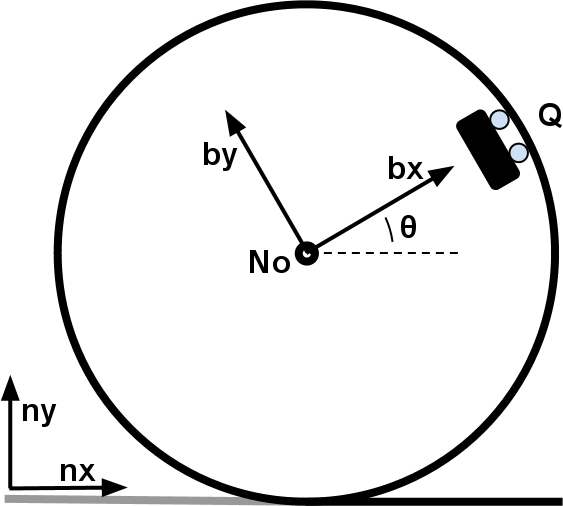
\includegraphics[width=0.85\textwidth]{RollerCoasterLoop.png}
\end{minipage}
%
%   \\[1.0pc] Neglecting air-resistance, the net force acting on Q due to gravity,
%   normal force from the track, and friction is
%   $\force{Q} = \minus[\;] mg \uvecy{n} \minus[\;] F_N \uvecx{b} \minus[\;] F_f \uvecy{b} $.

\begin{enumerate}
\setlength{\itemsep}{0.25pc}
%\item A sensor on the car measures its speed $v$ on the track, $v \deff[\;] \vel{Q}{N} \cdot \uvecy{b}$.
%      \\[0.0pc] Use this to complete the following table, solely in terms of the quantities listed at right:
%
%\begin{tabular}{|l|l|c|}
%           \hline Velocity of Q in N     & 	Acceleration of Q in N    & In terms of
%  \\[0.0pc]\hline  & &
%  \\[-0.5pc]       $\vel{Q}{N}   \equals[\;] \hspace{0.5cm}  R \thetadot \hfill \uvecy{b} \hspace{0.2cm}$
%                & $\accel{Q}{N} \equals[\;] \hidemath[0.7cm]{ \minus[\;] R \thetadot^2 } \uvecx{b} \plus[\;] \hidemath[0.9cm]{ R \thetaddot } \uvecy{b}$
%                & $R$, $\theta$, $\thetadot$
%  \\[1.0pc] \hline  & &
%  \\[0.5pc]       $\vel{Q}{N}   \equals[\;] \hidemath[0.9cm]{ v } \hfill \uvecy{b}  \hspace{0.2cm}$
%                & $\accel{Q}{N} \equals[\;] \hidemath[0.95cm]{ v^2 / R } \uvecx{b} \plus[\;] \hspace{0.9cm} \vdot \hfill \uvecy{b}$
%                & $R$, $v$, $\dot{v}$
%  \\[0.5pc]\hline
%\end{tabular}
\item Express $\vel{Q}{N}$ and $\accel{Q}{N}$ \textbf{efficiently},
      in terms of $R$, $\theta$, $\thetadot$, $\thetaddot$.
\vspace{2.5in}

\item  Use Newton's Law to write a \textbf{vector equation} describing the dynamics of Q \textbf{without} \thetadot, \thetaddot.
      %
      %\\[0.0pc]\textbf{Result:}\\[-1.45pc]

		\vspace{1.4in}

\clearpage
\item Dot your result from (b) with the appropriate unit vector to get a scalar equation of motion for the car that does \textbf{not} contain $F_N$. \textbf{Hint:} It may be helpful to write a rotation table.
\\[1.0pc]\textbf{Result:} \hspace{1in}  $\dot{v} = $
      \vspace{2.1in}

\item Dot your result from (b) with the appropriate unit vector to get a scalar equation for $F_N$ that does \textbf{not} contain $F_f$.
\\[1.0pc]\textbf{Result:} \hspace{1in}  $F_N = $
      \vspace{2.1in}

\item At its highest point ($\theta = 90^\circ$), how fast must the car travel so that the car (or a rider in it) feels \textbf{exactly} zero normal force?  Use your result from (d) and let $R = 10$ m and $g = 10$ m/s$^2$.
\\[1.0pc]\textbf{Result:} \hspace{1in}  $v = $
      \vspace{2.0in}

\item Based on your result from (e), explain if riders of higher mass must travel faster in order to avoid the tendancy to fall out of the roller coaster car.

\end{enumerate}
%
